\documentclass[preprint2]{aastex631}
\received{\today}
\shorttitle{Inside-Out Growth}
\graphicspath{{figures/}}

\usepackage{lipsum}
\usepackage{physics}
\usepackage{multirow}
\usepackage{xspace}
\usepackage{natbib}
\usepackage{fontawesome5}
\usepackage{xcolor}
\usepackage{wrapfig}
\usepackage[figuresright]{rotating}

% remove indents in footnotes 
\usepackage[hang,flushmargin]{footmisc} 

\newcommand{\todo}[1]{{\color{red}{[TODO: #1}]}}
\newcommand{\needcite}{{\color{magenta}{(needs citation)}}}
\newcommand{\placeholder}[1]{{\color{gray} \lipsum[#1]}}

% custom function for adding units
\makeatletter
\newcommand{\unit}[1]{%
    \,\mathrm{#1}\checknextarg}
\newcommand{\checknextarg}{\@ifnextchar\bgroup{\gobblenextarg}{}}
\newcommand{\gobblenextarg}[1]{\,\mathrm{#1}\@ifnextchar\bgroup{\gobblenextarg}{}}
\makeatother

\begin{document}

\title{{\Large Inside-Out Growth of Galaxies}\\\vspace{0.15cm}ASTR 511 Final Project}

% affiliations
\newcommand{\UW}{Department of Astronomy, University of Washington, Seattle, WA, 98195}

\author[0000-0001-6147-5761]{Tom Wagg}
\affiliation{\UW}

\correspondingauthor{Tom Wagg}
\email{tomwagg@uw.edu}

\section{Introduction}
For my project I'm going to investigate the inside-out growth of galaxies, focussing specifically on the Milky Way. This is the concept that star formation in spiral galaxies occurs first in the centre and builds outwards over time. This topic was first mentioned by Jim when we discussed chemical cartography and I decided to delve into the topic a bit more deeply (partially motivated by the fact that I used a model including inside-out growth in my paper \citep{Wagg+2022} and I didn't know what that was at the time).

\section{Background \& Early Simulations}
One of the first papers to propose the idea of inside-out growth was \citet{Larson+1976}. They extended previous simulations of galaxies with the goal of producing both a spheroidal and disc component to the galaxy. Most previous papers on the topic \citep[e.g.][]{Larson+1969, Gott+1973} focussed on reproducing the formation of elliptical galaxies and didn't investigate spiral galaxies with a significant disc component.

\citet{Larson+1976} start their simulations with a protogalaxy that is assumed to be a uniform, uniformly rotating sphere with a fixed total mass. Larson addresses the simplicity of these initial conditions by noting that, despite initial uniformity, collapse is always non-homologous and inhomogeneties still emerge.

They explore 9 different models of increasing complexity, including effects such as varying star formation rates, tidally inhibited star formation, different boundary radii. The final model that they find best fits the observations at the time uses a star formation rate that depends on the ratio of the cloud collision time to the free-fall time. This has the effect of producing a more realistic bulge to disc ratio.

\begin{figure}[htb]
    \centering
    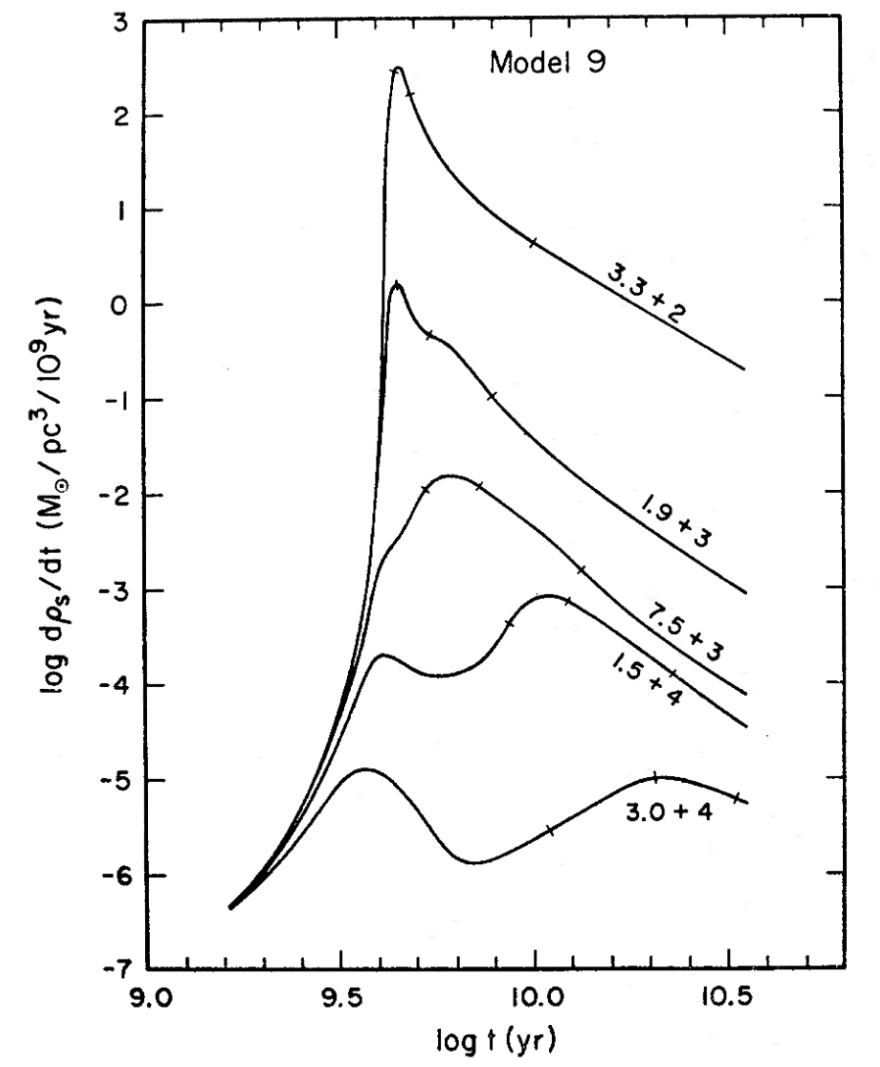
\includegraphics[width=\columnwidth]{larson1976_fig13.png}
    \caption{Figure 13 from \citet{Larson+1976}. This shows the star formation rate density as a function of time for different radii for Model 9 from the paper. Annotations indicate the radius, where for example $3.3+2$ means $3.3 \times 10^2$.}
    \label{fig:larson76}
\end{figure}

We show their modelled star formation rate density as a function of time and radius in Figure~\ref{fig:larson76}. They find that there are two distinct phases of star formation: an early burst that is centrally concentrated in the spheroidal component, and a later phase that occurs as gas settles into the plane of the disc. In particular, they note that this phase consists of ``an outward-progressing wave of star formation'' \citep{Larson+1976}. This is one of the first simulations showing a sort of ``inside-out'' growth.

They conclude that high velocity collisions between gas clouds may form spheroidal systems, whilst disc systems may form from more quiescent gas that doesn't require similar collisions. This gas settles onto the disc progressively over time, starting in the centre in which the potential is strongest and then progressing outwards.

\section{Observations}
\subsection{Evidence of inside-out growth}
Using data from 3D-HST and CANDELS Treasury surveys, \citet{vanDokkum+2013} investigated the assembly of Milky-Way-like galaxies since redshift 2.5.

They use the number density of galaxies to rank them and assume that galaxies maintain the same rank throughout cosmic time. This has been shown to be a reasonably effective way of associating progenitor galaxies with their descendants \citep{Leja+2013}. They select galaxies with stellar masses close to that of the Milky Way and use this ranking method to associate galaxies together in order to measure their evolution over time. This produces a sample of approximately 400 galaxies.

\begin{figure}[htb]
    \centering
    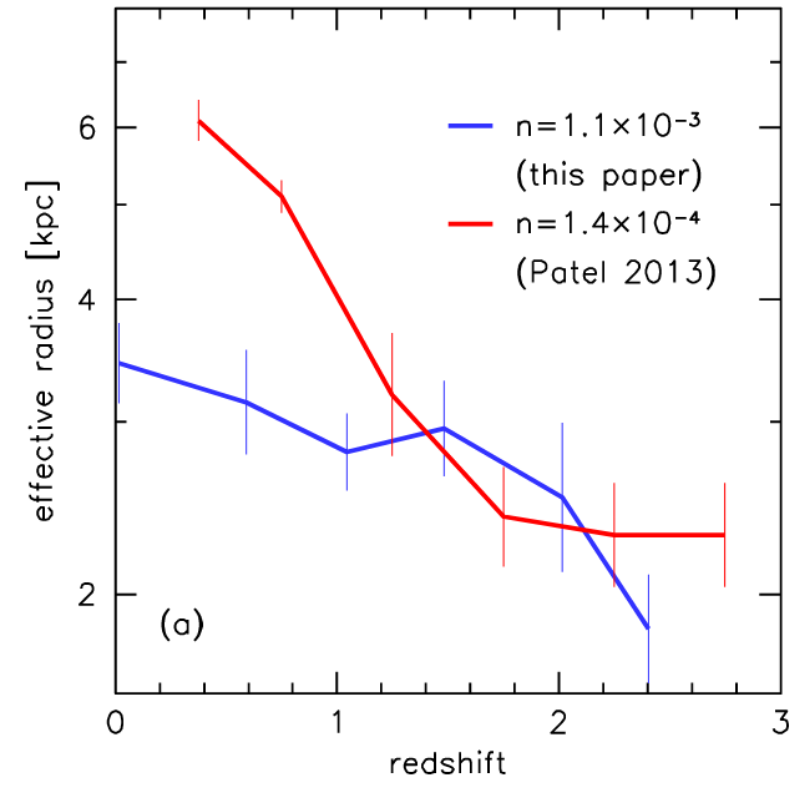
\includegraphics[width=\columnwidth]{vandokkum2013_fig5.png}
    \caption{Figure 5 from \citet{vanDokkum+2013}. The effective radius of observed galaxies from 3D-HST and CANDELS at different redshifts, compared to another paper.}
    \label{fig:vd}
\end{figure}

After grouping galaxies into bins of redshit, \citet{vanDokkum+2013} stack galaxies and fit them using a \citet{Sersic+1968} profile (correcting for PSF effects and bootstrapping to produce error bars). We show their estimated effective radii for galaxies of different redshifts in Figure~\ref{fig:vd}.

Figure~\ref{fig:vd} shows that the effective radius of a galaxies decreases with increasing redshift, implying that galaxies are growing over time and thus providing evidence for some sort of inside-out growth. It is also notable that within this figure they also compare to \citet{Patel+2013}, a paper that finds stronger evidence of inside-out growth in more massive galaxies. They conclude that there is likely some sort of mass dependence to the rate of inside-out growth and that galaxy formation models will need to explain both effects.

\subsection{A lack of evidence}
\citep{Goddard+2017}

\begin{figure*}[t]
    \centering
    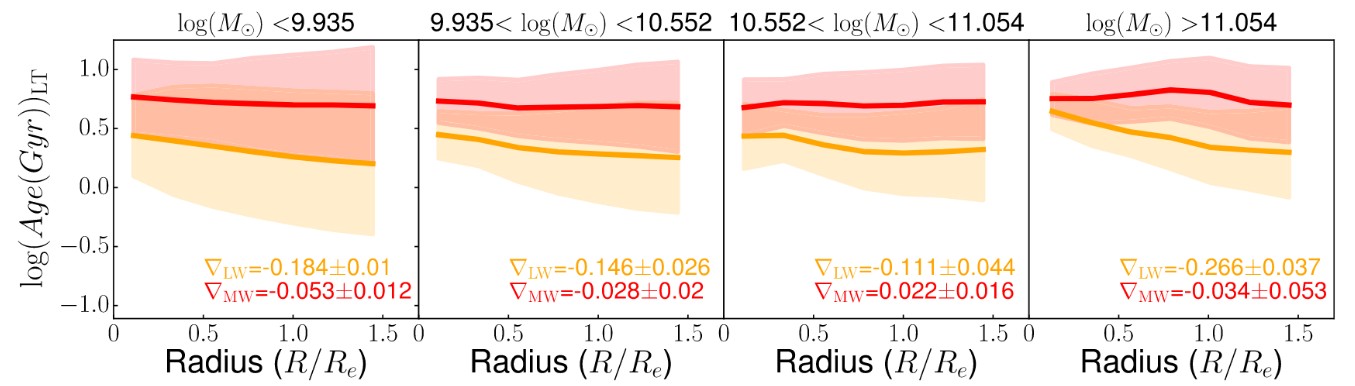
\includegraphics[width=\textwidth]{goddard2017_fig14.png}
    \caption{Figure 14 from \citet{Goddard+2017}. Mass weighted age-radius gradients are given in red for four different mass bins, from observations in SDSS-IV MaNGA.}
\end{figure*}

\section{Models}
\citep{Frankel+2019}

\section{Applications}
\citep{Banerjee+2020}

\section{Future Work}
\citep{Hogg+2019}

\begin{figure}[htb]
    \centering
    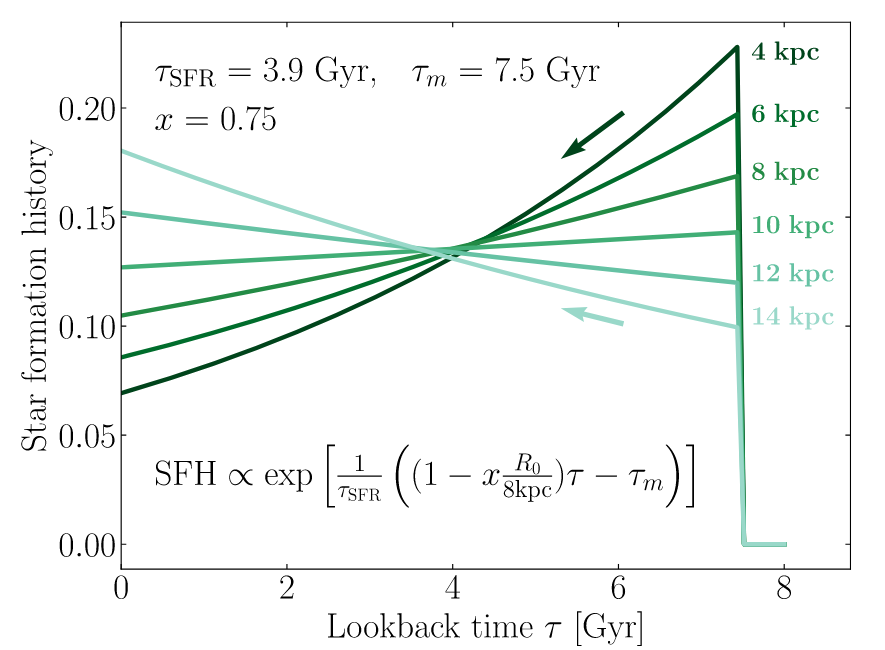
\includegraphics[width=\columnwidth]{frankel2019_fig5.png}
    \caption{\citet{Frankel+2019} Figure 5 showing the model for inside-out growth.}
\end{figure}

\begin{figure}[htb]
    \centering
    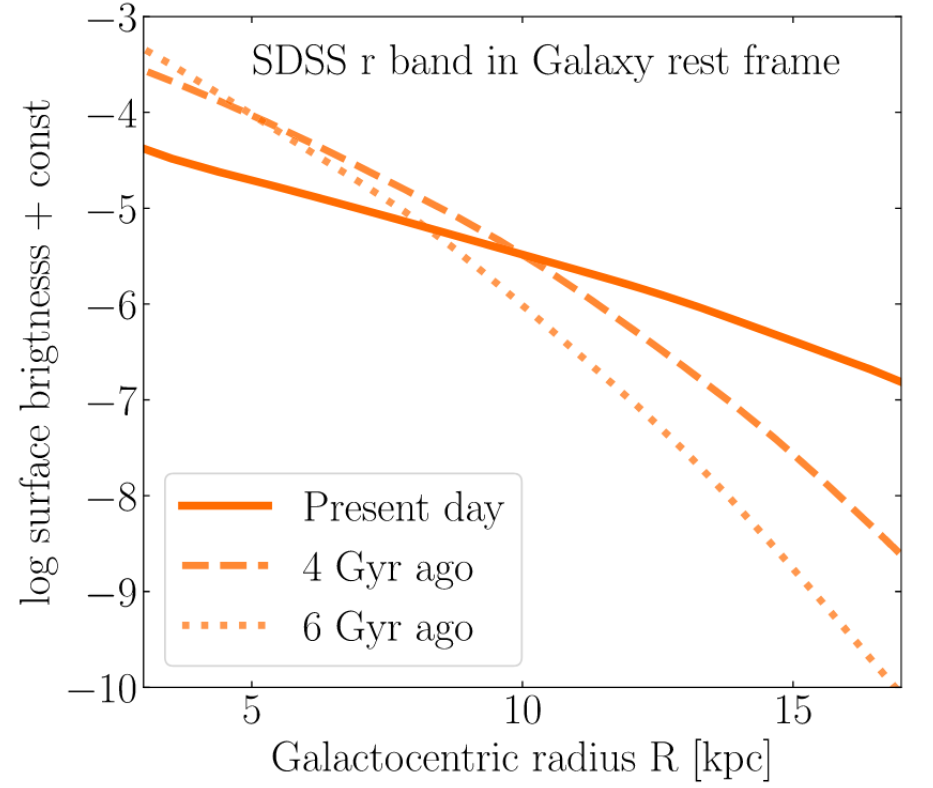
\includegraphics[width=\columnwidth]{frankel2019_fig9.png}
    \caption{}
\end{figure}

\begin{figure}[htb]
    \centering
    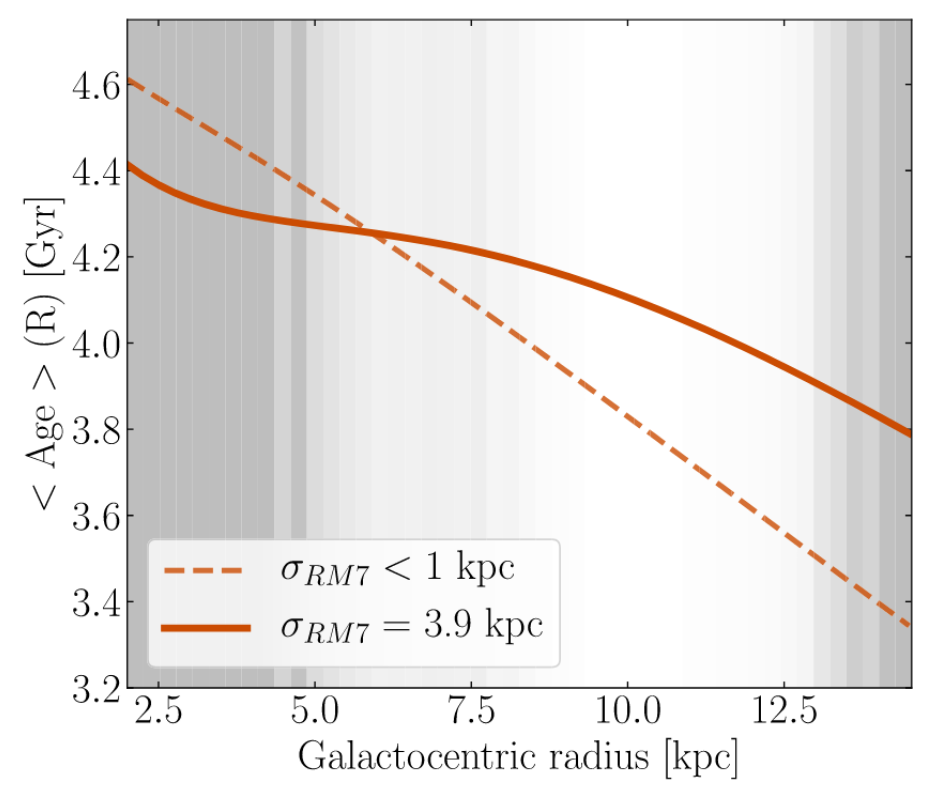
\includegraphics[width=\columnwidth]{frankel2019_fig12.png}
    \caption{}
\end{figure}

\begin{acknowledgements}
    I thank my laptop for not losing any data despite the fan malfunctioning and the whole thing nearly exploding and I thank GitHub for having my back on that just in case. Since this is acknowledgements, I will also acknowledge that this isn't my very best work, but it's been quite the quarter and I would like to sleep now :D
\end{acknowledgements}

\bibliographystyle{aasjournal}
\bibliography{refs}{}

\end{document}